% !TEX root = ../main.tex

% TODO inform dietrich of the Technologies/Structure switch

\chapter{Technologies used}
\label{ch:technologiesUsed}

In this chapter, technologies used in the project and subsequently shown in code samples in later chapters will be introduced.
This enables a better understanding of the code samples and comprehension of the underlying theory.\\
Technologies like libraries and frameworks that are specific to certain methodologies,
meaning that they are or contain the implementation of said methodologies,
and are only used for that implementation,
will be explained in the respective methodologies's section of this thesis.\\
Furthermore, the technologies used for the dashboard will only be explained in the respective chapter,
since the dashboard is only used for the interaction with and visualization of the underlying analysis,
not for the analysis itself.

\section{Languages}
\label{sec:languages}

Only the Python programming language was used, since it is general-purpose,
has a high level of abstraction and focuses on readability,
which will be beneficial when working with complex architectures and algorithms later on~\cite{pythonDocs}.
Python follows multiple paradigms.
It is object-oriented, imperative, procedural and reflective~\cite{van2007python}.
It also supports dynamic typing, which enables its users to focus on higher-level tasks, at the cost of computational efficiency \cite{Perez-schofield2010}.
Since its inital release in 1991, these and more aspects have made it a popular choice among researches.
As seen in~\ref{table:python}, there are currently 2 supported versions of Python, which are not backwards compatible.
In this thesis, version 3.6.2 is used.
Furthermore, virtualenv was used to make the development environment easily reproducible on other machines.

% TODO ask dietrich how to properly cite this excerpt from van2007python, since some part are just copied over
\begin{table}
    \caption{The Python programming language~\cite{van2007python}}
    \label{table:python}
    \vspace{0.2cm}
    \begin{tabular}{l | l} %
        Paradigms
        & Multi-paradigm: object-oriented, imperative, functional,
        \\ & procedural, reflective
        \\ \midrule
        Appeared in
        & 1991
        \\ \midrule
        Designed by
        & Guido van Rossum
        % TODO properly link to his name
        \\ \midrule
        Developer
        & Python Software Foundation
        % TODO properly link to the Python software foundation
        \\ \midrule
        Stable releases
        & 3.6.2 and 2.7.13 (8. September 2017)
        \\ \midrule
        Typing discipline
        & duck, dynamic, strong
        \\ \midrule
        OS
        & cross-platform
        \\ \midrule
        Usual filename extensions
        & .py, .pyw, .pyc, .pyo, .pyd
    \end{tabular}
\end{table}

% TODO maybe also talk about other languages considered, with comparison table


\section{Libraries}
\label{sec:libraries}

\subsection{Kafka}
\label{subsec:kafka}

Kafka is a distributed messaging system implementing the publish/subscribe paradigm.
In the publish/subscribe paradigm, subscribers register their interest in a certain type of event,
and are asynchronously notified by the system when an event is published that matches the criteria~\cite{Eugster2003}.
In Kafka, the publishing entities are called producers, and the subscribing entities are called consumers.
A stream of events (called messages in Kafka) of a particular type that a consumer can subscribe to is defined by a topic~\cite{Kreps2015}.

% include diagram
\begin{figure}
    \centering
    \caption{Simplified diagram of a typical Kafka setup.}
    \label{fig:kafka}
    % TODO smaller maybe it somehow fits next to the python table.
    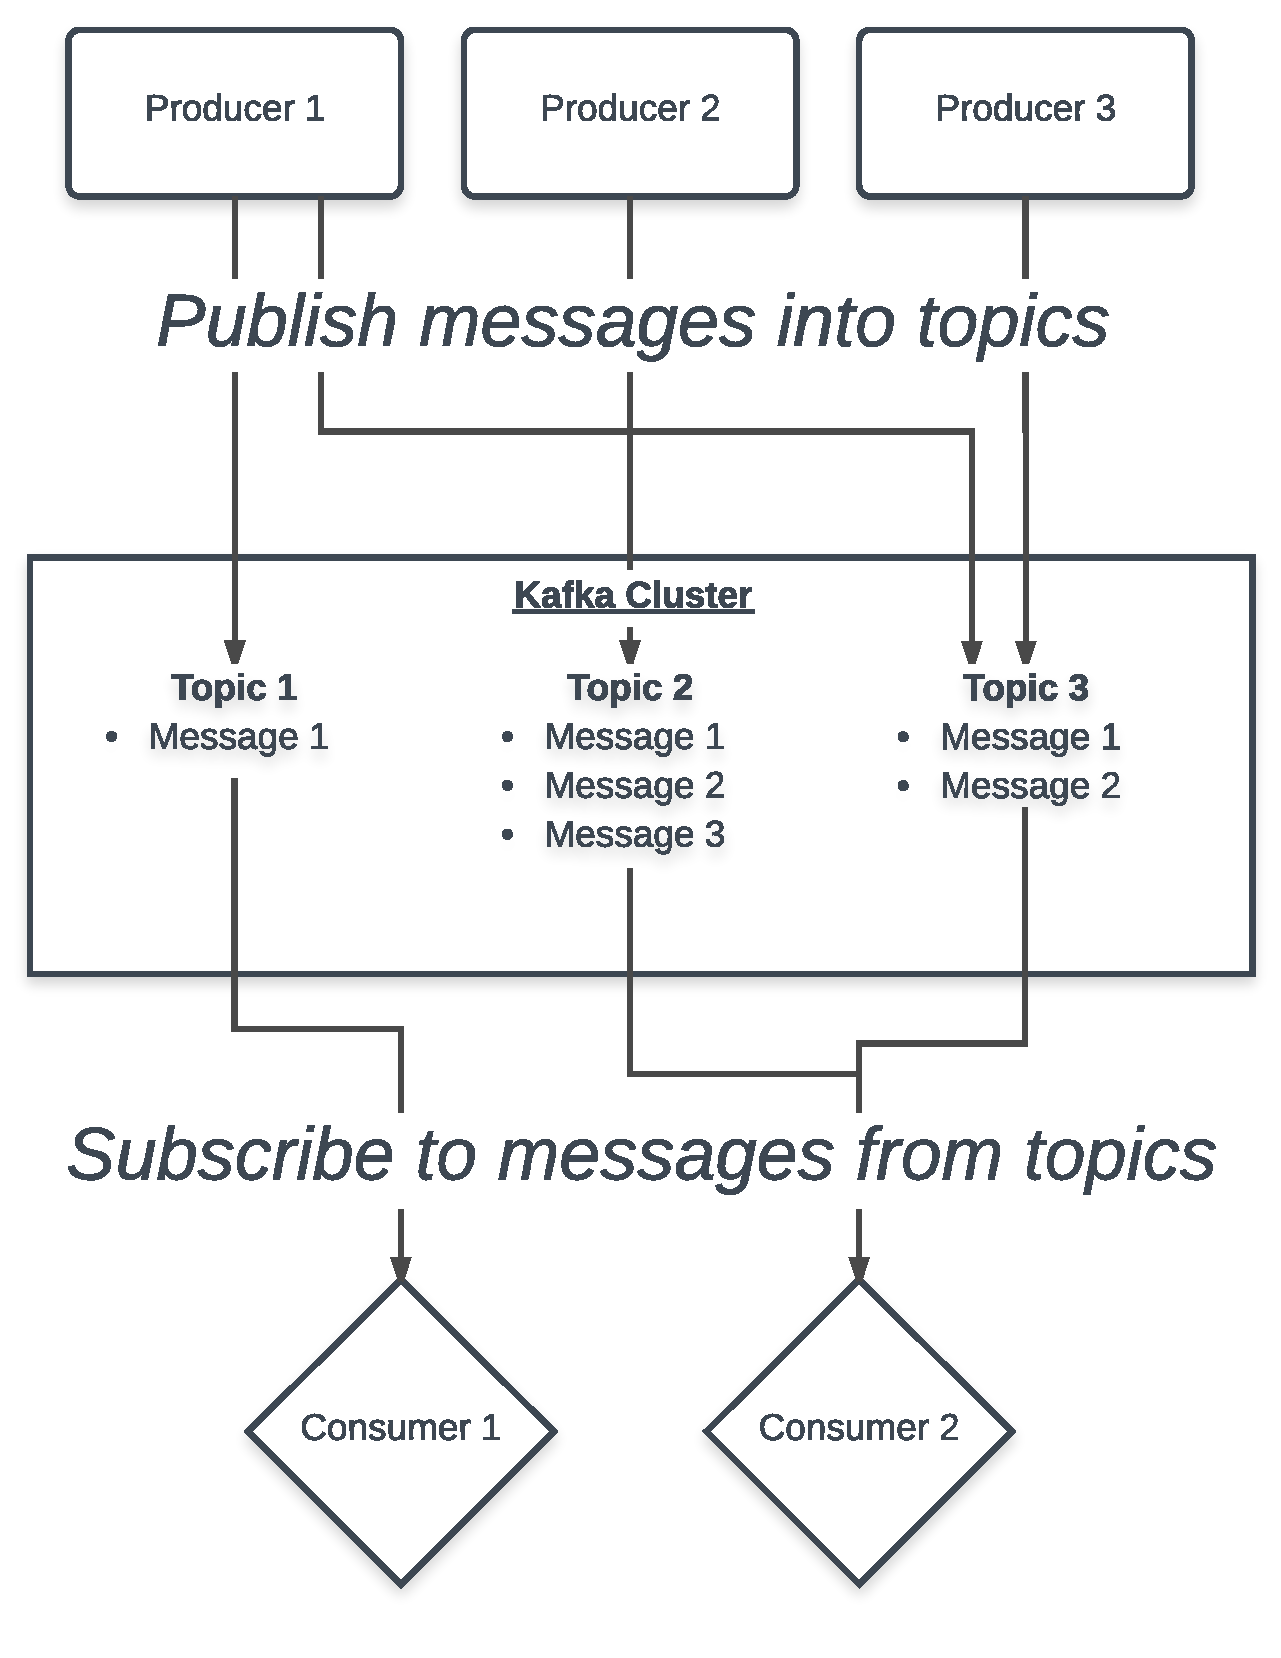
\includegraphics[width=\textwidth]{../figures/kafka.pdf}
\end{figure}

\ref{fig:kafka} shows a simplified, typical configuration of a messaging system powered by Kafka.
The Kafka cluster is a set of message brokers, being replicated and running on different machines, that can each contain messages for every topic,
which are then distributed to the subscribing consumers~\cite{Kreps2015}.
The system scales vertically, enabling high throughput and redundance.

% Figure and Code example
\subsection{Spark}
\label{subsec:spark}

% Whats the problem?
The amount of data being processed when streaming social network data,
especially with multiple users and when streaming a broad set of activities,
commands large amounts of computing power that cannot be provided by solely scaling up,
meaning increasing the performance of a single machine.
Instead, the performance required is achieved by scaling out,
meaning distributing the computation across multiple machines~\cite{Wolke2010}.
\par % Spark solves it!
Spark manages this scaling out by abstracting these machines as so-called execution nodes (also called worker nodes or slave nodes),
on which programs (tasks) called sparkjobs are run.
These abstract execution nodes can also be separate processes on a single machine,
efficiently utilizing multiple cores. % TODO maybe a screencap of many python processes
The distribution of tasks to these nodes, and the collection of results from them,
is managed by the master node (also called driver node).
It utilizes Apache Hadoop to persist data across these nodes~\cite{Zaharia2016}.
\ref{fig:spark} illustrates this architecture.

% include diagram
\begin{figure}
    \centering
    \caption{Simplified diagram of a typical Spark cluster}
    \label{fig:spark}
    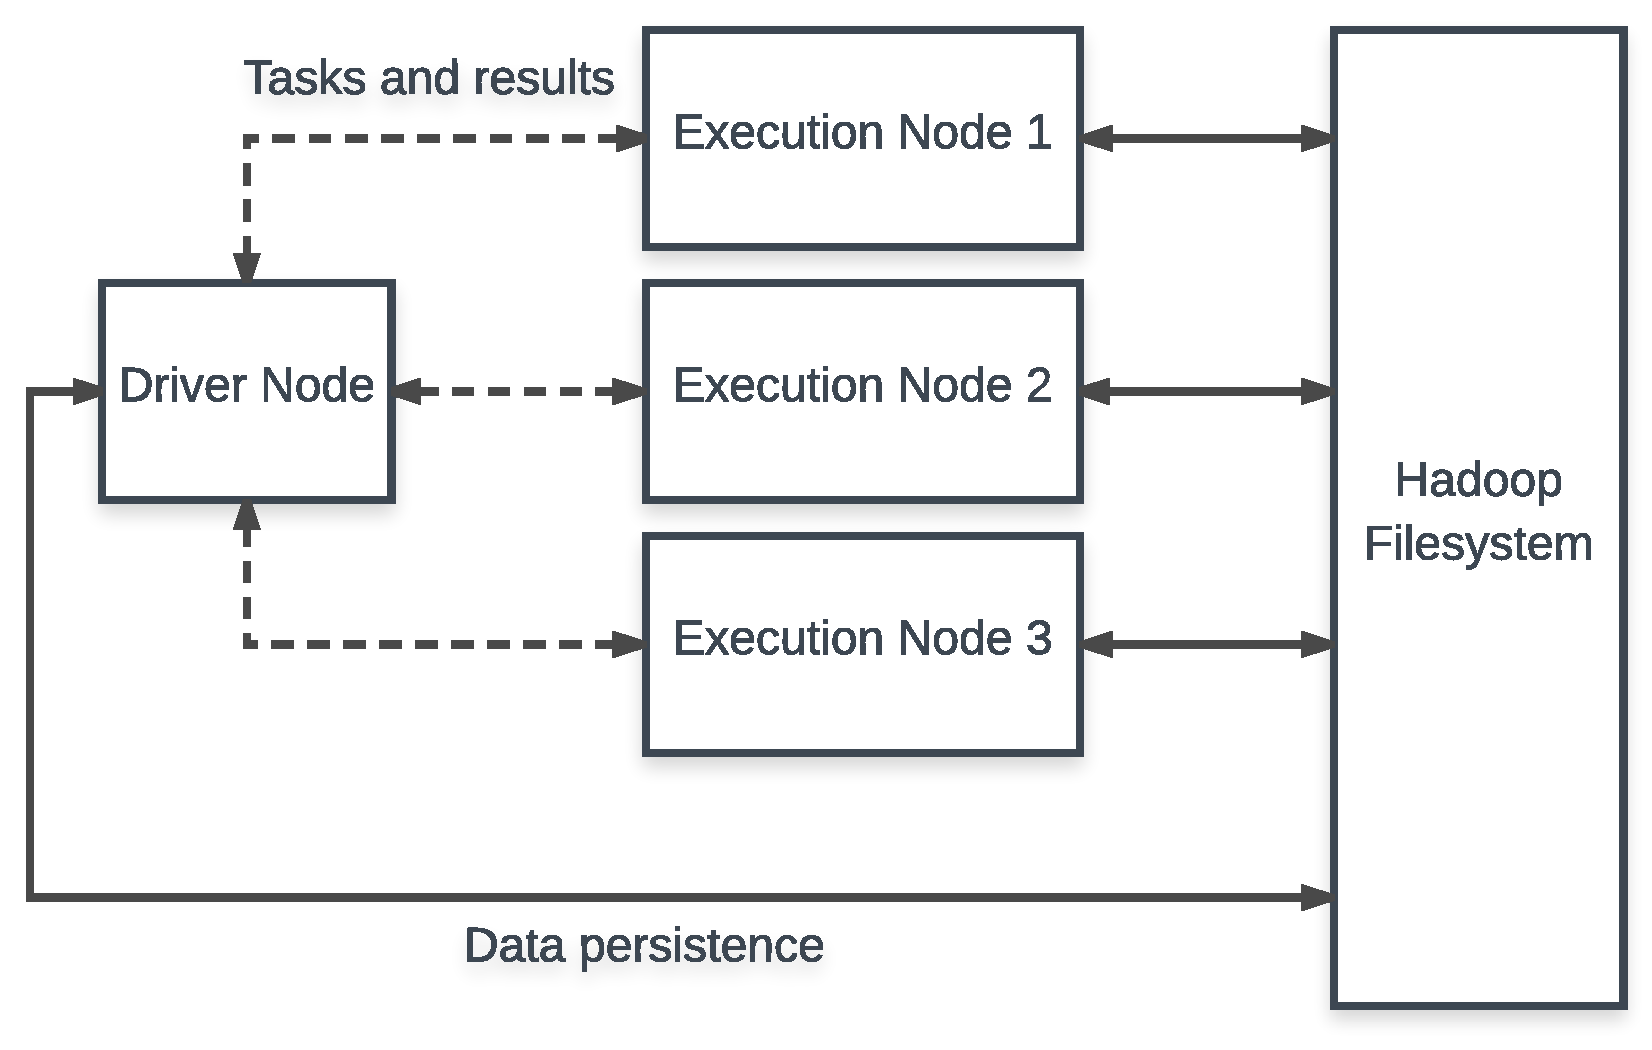
\includegraphics[width=10cm]{../figures/spark.pdf}
\end{figure}

\par
Spark also offers functionality to perform machine learning, data analysis and more on data from streams,
files or databases, in a distributed setting, with just a few lines of code~\cite{sparkDocs}.
This means that Spark unifies and simplifies a lot of tasks in one framework that previously required multiple technologies.
This has lead to a widespread adoption of Spark since its release in 2010,
making it the biggest open source big data project~\cite{Zaharia2016}, with over 1100 contributors~\cite{sparkContributor}.

% How does it do such magic? Going under the hood
\par
Spark uses a concept called RDDs
(\textbf{R}esilient \textbf{D}istributed \textbf{D}atasets),
through which the parallelization, distribution and persistence of data is abstracted for the developer~\cite{sparkDocs}, see ~\ref{code:simpleParallelization} for a simple example.

\begin{figure}
    \caption{A simple example showing how spark distributes data and collects the result back to the driver node (~\cite{sparkDocs}, modified)}
    \label{code:simpleParallelization}
    \begin{minted}{python}
        % @formatter:off
data = [1, 2, 3, 4, 5]
# Wrap the data into a RDD, which is distributed across execution nodes by Spark, ready for parallel processing
# sc is the so-called streaming context, which provides an interface with the cluster
distributedData = sc.parallelize(data)
# Add a map-action that increments each value, distributed across execution nodes
incrementedData = distributedData.map(lambda a: a + 1)
# Run a reduce-transformation, which is run on the driver node
# The RDD is automatically collected (persisted) to the driver node
incrementedData.reduce(lambda a, b: a + b)
# returns 20
            % @formatter:on
    \end{minted}
\end{figure}

Furthermore, Spark is developed by the Apache Software Foundation, as is Kafka,
which means they are designed to work well with each other.
For example, the Python API of Spark offers a range of utility functions to build sparkjobs to consume a Kafka-stream very easily~\cite{sparkDocs}.
which means constructing a sparkjob to act as a consumer for a Kafka-stream in a distributed setting can be achieved with very few lines of code,
as can be seen in the wordcount-example in~\ref{code:wordcount}.

\begin{figure}
    \caption{Consuming data from a stream and processing them in batches}
    \label{code:wordcount}
    \begin{minted}{python}
        % @formatter:off
# Stream the data in 1-second windows
streaming_context = StreamingContext(sc, 1)  # 1 second window
# Connect to a kafka stream, specifying which kafka-topics to consume. See section "Kafka" for an explanation of topics.
stream = KafkaUtils.createStream(streaming_context, 'docker:2181', "stream-1", {"topic-1": 1})
# Each window, count each word in each line
counts = stream.flatMap(lambda line: line.split(" ")) \
    .map(lambda word: (word, 1)) \
    .reduceByKey(lambda a, b: a + b)
            % @formatter:on
    \end{minted}
\end{figure}

Spark also allows for more complex functions to be applied to the data.
The previous examples~\ref{code:simpleParallelization} and~\ref{code:wordcount} exclusively used lambda expressions~\cite{pythonDocs},
however, not all functions can be expressed as a lambda expression.
Also, developers might need to use variables defined outside of the function because their initialization is computationally intensive,
or use data that is only available on the driver node.
One real strength of spark is that it can transmit variables used in a function, but defined outside of it, to the execution nodes, as long as they are serializable~\cite{sparkDocs}.
This also includes imported packages, which enables developers to very easily use other libraries and frameworks on the execution nodes.
Since one of Pythons paradigms is functional programming~\ref{sec:languages},
the factory-pattern was used in this thesis to create the functions executed on the execution nodes along with variables and packages used in it.
A simple example of this can be seen in~\ref{code:factory}.

\begin{figure}
    \caption{Demonstration of using packages and outside-variables on execution nodes}
    \label{code:factory}
    \begin{minted}{python}
        % @formatter:off
# Factory to create a match-function that matches a text against a compiled regular expression
def matcher(pattern):
    # imports...
    import re
    # ...and variables...
    compiled = re.compile(pattern)

    def match(text):
        # ...are serialized and transmitted to the execution node to be used in the function
        return re.match(compiled, text)

    return match

# Usage:
someRDD.map(matcher("ab*"))
            % @formatter:on
        %TODO can man den code safe einrücken ohne dass es die Darstellung kaputt macht? Ausprobieren
    \end{minted}
\end{figure}

\subsection{NLTK}
\label{subsec:nltk}

The NLTK (\textbf{N}atural \textbf{L}anguage \textbf{T}ool\textbf{K}it) is a Python-toolkit consisting of several libraries used for
natural language processing.
It interfaces with many lexical resources and corpora, and offers functions for tokenizing, stemming and parsing text-based artifacts,
and many more~\cite{nltkDocs}.
The NLTK is mainly used by students, teachers and researchers, as a self-study tool or for teaching,
and to prototype and build research systems such as this thesis.
The community appreciates the shallow learning curve and that it is unopinionated~\cite{Bird2006}.
It was used across the project of this thesis for utilitarian and miscellaneous tasks.
A simple exemplary use-case can be seen in~\ref{code:nltk}.

\begin{figure}
    \caption{Example usage of the NLTK in a Python shell}
    \label{code:nltk}
    \begin{minted}{python}
        % @formatter:off
import nltk
text = "the quick brown fox jumps over the lazy dog"
# The NLTK offers, for example, word tokenization
tokens = nltk.tokenize.word_tokenize(text)
tokens
Out[3]: ['the', 'quick', 'brown', 'fox', 'jumps', 'over', 'the', 'lazy', 'dog']
# It also offers a wrapper-class for text that enables, for example, searching it and displaying the results.
wrapped = nltk.Text(tokens)
wrapped.concordance("fox")
Displaying 1 of 1 matches:
                      the quick brown fox jumps over the lazy dog
            % @formatter:on
        %TODO can man den code safe einrücken ohne dass es die Darstellung kaputt macht? Ausprobieren
    \end{minted}
\end{figure}

Some of the more complex functionality and methods for classification that border on machine learning territory were also used,
although they are explained in more detail in their respective chapters~\ref{ch:sentimentAnalysis}.

\section{Project Structure}
\label{sec:projectStructure}

As with any programming project, high-quality, well documented and structured code is important this thesis.
Since the programming language used in this thesis is Python, and it is in large parts data-science,
the "Cookiecutter Data Science" %TODO quote properly
project structure is used~\cite{dsCookieCutter}.
This project structure follows a type-based separation, an explanation of the individual folders can be seen in~\ref{forest:dscookiecutter}.

% TODO use the folder icon in all forest https://tex.stackexchange.com/questions/5073/making-a-simple-directory-tree
\begin{figure}
    \caption{The folder structure of the "Cookiecutter Data Science"~\cite{dsCookieCutter}} %TODO quote properly
    \label{forest:dscookiecutter}
    \begin{forest}
        % @formatter:off
% TODO can this be safely indented? same as code
  for tree={
    font=\ttfamily,
    grow'=0,
    child anchor=west,
    parent anchor=south,
    anchor=west,
    calign=first,
    edge path={
      \noexpand\path [draw, \forestoption{edge}]
      (!u.south west) +(7.5pt,0) |- node[fill,inner sep=1.25pt] {} (.child anchor)\forestoption{edge label};
    },
    before typesetting nodes={
      if n=1
        {insert before={[,phantom]}}
        {}
    },
    fit=band,
    before computing xy={l=15pt},
  }
[Thesis
  [data \textit{all data}
    [external \textit{data from external sources}
    ]
    [interim \textit{data that has started\, but not finished processing}
    ]
    [processed \textit{data that is ready to be used}
    ]
    [raw \textit{collected\, yet unprocessed data}
    ]
  ]
  [docs \textit{documentation of the project}
  ]
  [models \textit{trained model binaries}
  ]
  [notebooks \textit{Jupyter notebooks used for exploration}
  ]
  [references \textit{references and attributions for the code}
  ]
  [reports \textit{written reports such as this thesis}
  ]
  [src \textit{all code}
    [data \textit{code related to acquisition and processing of data}
    ]
    [models \textit{code related to training the models}
    ]
    [streaming \textit{code used for streaming data}
    ]
    [visualization \textit{code used to visualize results}
    ]
  ]
]
        % @formatter:on
    \end{forest}
\end{figure}
% TODO maybe uncomment this and remove the references directory from the forest above
% Since few of the externally sourced parts of code required attribution, and there was little previous work to reference in code, the \texttt{/references} directory remained unused and was removed.
Additionally, a \texttt{/streaming} directory was created under \texttt{/src}, which accommodates all streaming-related modules.
Beyond the structure given by the cookie cutter, further down in the directory tree, feature-based separation is employed,
to make the code easily expandable with further analysis and modeling beyond what is implemented in this thesis.
A part of the folder structure showcasing this project structure can be seen in the \texttt{notebooks} directive, shown in~\ref{forest:featurebased}.


% another forest


Using the DS cookie cutter, except the streaming folder is one under source because it is used by data to collect training data and by visualization for the dashboard.
Generally a modular approach that can be easily expanded with further analysis/monitoring beyond the LDA/Sentiment Analysis with Naive Bayes combination has been build.


\section{Architecture}
\label{sec:architecture}

Explaining the choice of architecture with some figures.
% TODO architecture diagram from the book
Explaining how all the previously mentioned technologies work together

Processing Data in motion, page 49

In our case, we only have one execution node, but Kafka and Spark are designed such that there should not be a problem with more nodes

% TODO do this at then end, its not perfectly clear what to put here right now